\begin{titlepage}		% titlepage is a special environment, which is defined between this command and the corresponding \end{titlepage} command

	% suppress error "destination with the same identifier" ...
  \setcounter{page}{-1}			% to have the page counter showing 1 for the first actual page after the titlepages

\begin{center}


% Upper part of the page

\textsc{\Large Polar Ocean Climate AGF-214}\\[0.5cm]


% Title
\newcommand{\HRule}{\rule{\linewidth}{0.5mm}}
\HRule \\[0.4cm]
{ \huge \bfseries Field Report 2022}\\
\HRule \\[1.5cm]
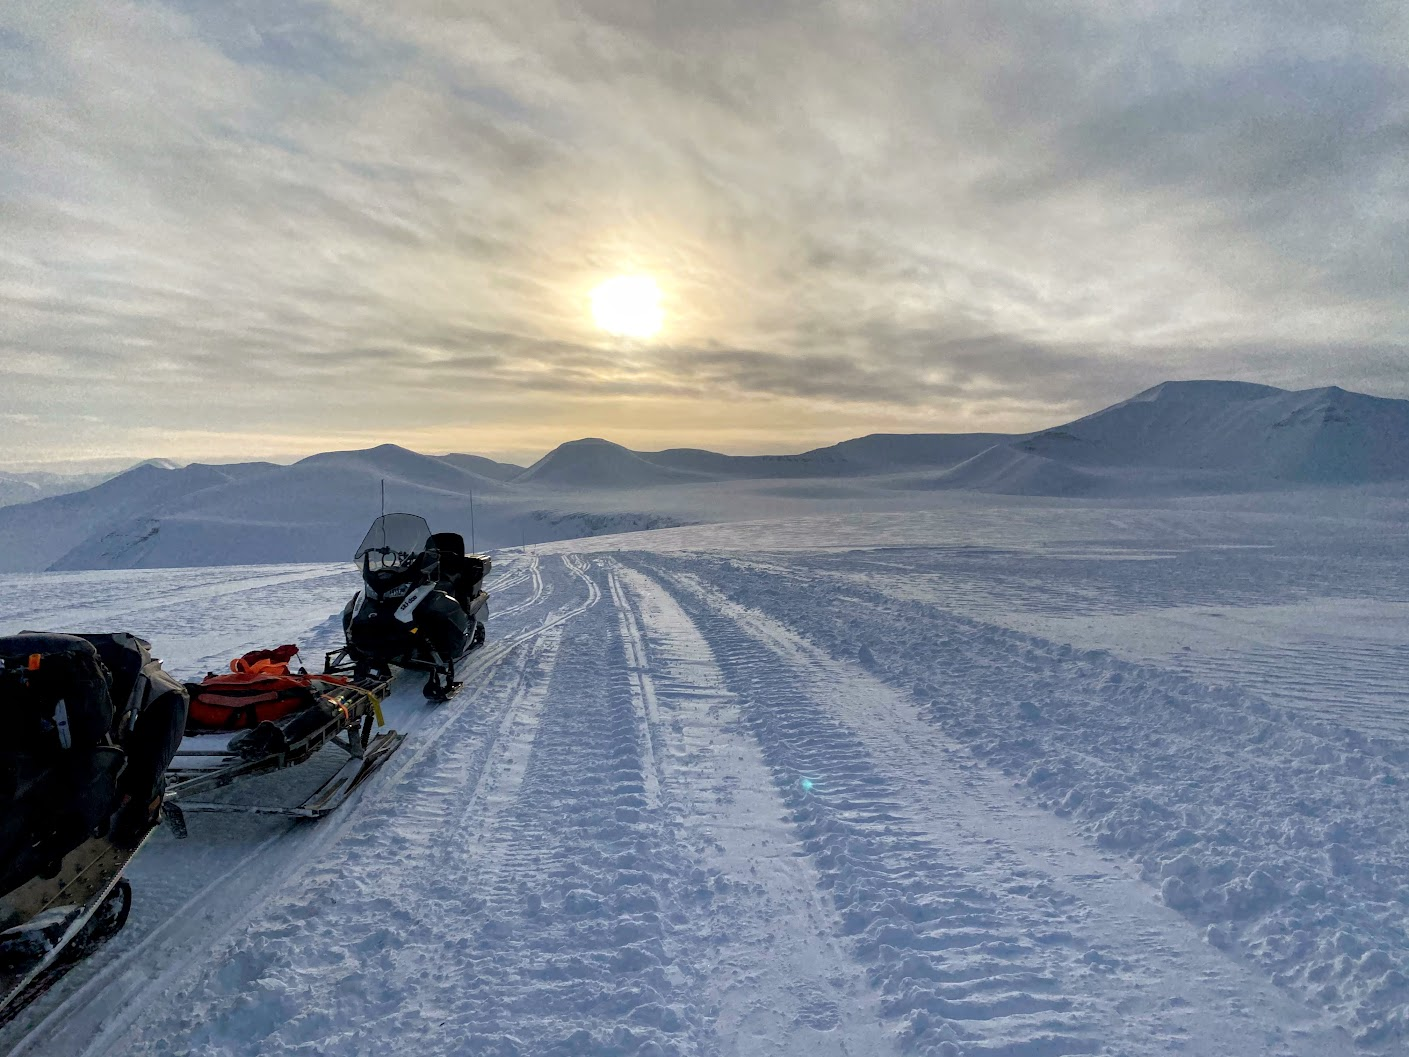
\includegraphics[width=0.8\textwidth]{./figures_main/cover_image} % if there are more than just one image, they should be merged in a graphic program like GIMP beforehand.

\vfill

% Author and supervisor

\emph{Authors:}\\
John Lennon, Paul McCartney, Mary Poppins, Mark Twain

\vspace{1cm}

\emph{Instructors:}\\
Moby Dick, Nils Holgerson


\vfill

% Bottom of the page

\includegraphics[width=0.3\textwidth]{./figures_main/unis_logo}

\end{center}

\newpage
\thispagestyle{empty}			% to suppress the header and footer lines for the title pages

\end{titlepage}

